\title{CS 301, Course Project - Report} % You may change the title if you want.
% \subtitle{Hello}
\author{Abhishek Raj (180010002), Harsh Raj (180010017), Rishit Saiya (180010027)}

\date{\today}

\documentclass[12pt]{article}
\usepackage{fullpage}
\usepackage{enumitem}
\usepackage{amsmath,mathtools}
\usepackage{amssymb}
\usepackage[super]{nth}
\usepackage{textcomp}
\usepackage{hyperref}
\hypersetup{
    colorlinks=true,
    linkcolor=blue,
    filecolor=magenta,      
    urlcolor=cyan,
}
\begin{document}
\maketitle

%---------------------------------------------------------------------

\section{Abstract}
The report touches upon an \href{https://en.wikipedia.org/wiki/ARM_architecture}{ARM} project where we are given an array of unpacked BCD numbers are stored starting from memory location U\_BCD. We have converted the unpacked BCD numbers to packed BCD numbers and stored the array starting from memory location P\_BCD.

We have also explained upon some the problem statements explaining in detail about parameters like Number of Static \& Dynamic Instructions, Instruction Counts under various constraints, Code Coverage, Execution Time, etc. It also explains in details of our previous versions/ideas and the breakpoints where we chose a different idea to enhance and achieve the results. \\


\textbf{Note about Codes:} \\
    \textbf{\textit{main.s}} contains the main ARM code (This code is written without conditional execution). \textbf{\textit{main\_thumb.s}} contains the code using THUMB instructions.
%---------------------------------------------------------------------

\section{Simulator \& Software Dependencies}

ARM Assembly Language Programming is used to code in the \textbf{.asm} file.
We are using \href{https://www.nxp.com/docs/en/data-sheet/LPC1769_68_67_66_65_64_63.pdf}{NXP’s ARM Cortex M3 – LPC1768} for simulation of our program. All the statistics mentioned in this report are in state-of-art to the software packs for LPC1768 updates to this date.
We have performed simulation using \href{https://www.keil.com}{Keil SDE} which provides a wide range of ARM Cortex-M based microcontroller devices.
%---------------------------------------------------------------------

\section{Q.1 - Static \& Dynamic Instructions}
The basic definitions of Static \& Dynamic Instructions are as follows: \\

\textbf{\textit{Static Instruction:}} The number of instructions of the program will constitute number of Static Instructions. \\
The number of Static Instructions of our code is \textbf{\textit{20}}.

\textbf{\textit{Dynamic Instruction:}} The actual number of instructions executed by the CPU for a specific program execution will constitute as number of Dynamic Instructions. \\

The generalised expression for number of Dynamic Instructions is as follows: \\
\begin{equation*}
    Dynamic \, Instructions = \frac{5n^{2} + 29n}{2} + 9
\end{equation*}
where n is the number of unpacked BCD numbers in an array

%---------------------------------------------------------------------

\section{Q.2 - Instruction Counts under various Constraints}
\begin{enumerate}[label=(\alph*)]
    \item The number of Instruction Counts when code without conditional execution was involved is \textbf{\textit{20}}.
    \item By usage of Conditional Execution in our code, we observed that there was no change in number of instructions than previous but there were instances where it could increase. So we avoid that.
    \item We observed that when code written with THUMB instructions was implemented, the code execution time dropped which is a sign of an efficient implementation. Upon seeing the reason, we came to know that it happens so due to reduced number of instructions along with less variation in values of flags.
    The number of instructions in this case was \textbf{\textit{17}}. \\
    
    Figure 1 further approves towards the fact that with Thumb Instruction, the code execution took \textbf{3.833 µs} whereas without Thumb Instructions, the code execution took \textbf{5.250 µs}.
    \begin{center}
    \begin{figure}
        \centering
        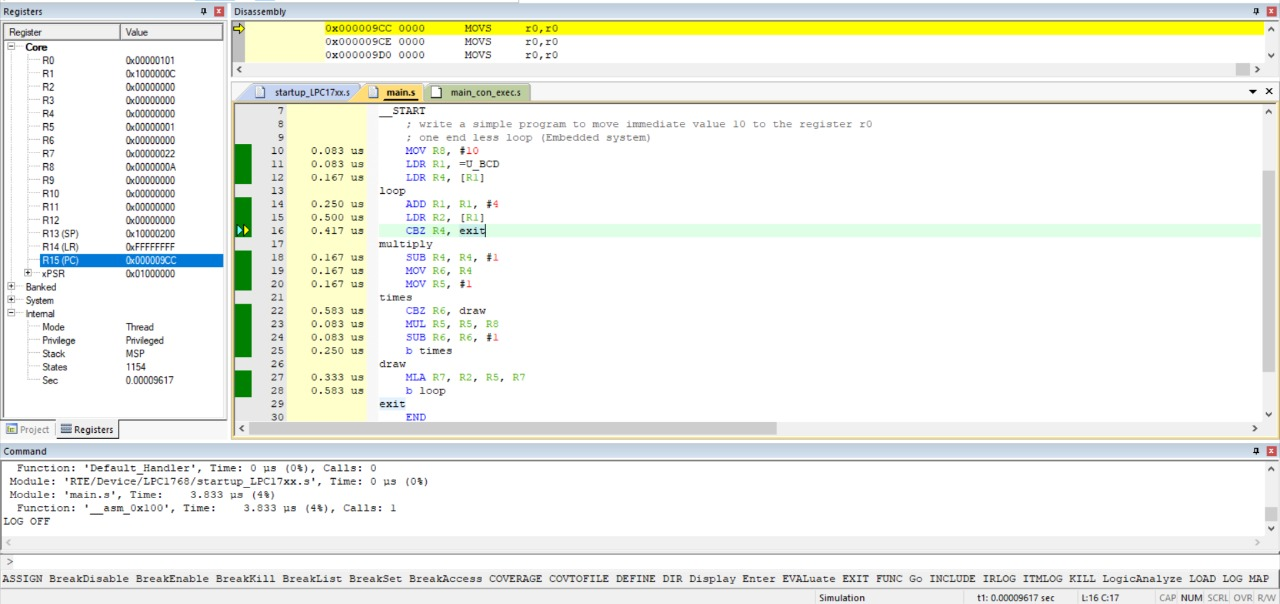
\includegraphics[width=15cm, height=8cm]{Course Project/Thumb.png}
        \caption{Screenshot of code using THUMB instructions showing its execution time is less}
    \end{figure}
\end{center}
    
\end{enumerate}

%---------------------------------------------------------------------

\section{Q.3 - Code Coverage, Code Execution Time, No. of Calls Executed}
\begin{enumerate}[label=(\alph*)]
    \item The code coverage and its contents were migrated into a file \textbf{mainlog} whose contents are as follows:
    \begin{verbatim}
\\project\RTE/Device/LPC1768/startup_LPC17xx.s\Reset_Handler - 
100% (2 of 2 instructions executed)
\\project\RTE/Device/LPC1768/startup_LPC17xx.s\NMI_Handler - 
0% (0 of 1 instructions executed)
\\project\RTE/Device/LPC1768/startup_LPC17xx.s\HardFault_Handler - 
0% (0 of 1 instructions executed)
\\project\RTE/Device/LPC1768/startup_LPC17xx.s\MemManage_Handler - 
0% (0 of 1 instructions executed)
\\project\RTE/Device/LPC1768/startup_LPC17xx.s\BusFault_Handler - 
0% (0 of 1 instructions executed)
\\project\RTE/Device/LPC1768/startup_LPC17xx.s\UsageFault_Handler - 
0% (0 of 1 instructions executed)
\\project\RTE/Device/LPC1768/startup_LPC17xx.s\SVC_Handler - 
0% (0 of 1 instructions executed)
\\project\RTE/Device/LPC1768/startup_LPC17xx.s\DebugMon_Handler - 
0% (0 of 1 instructions executed)
\\project\RTE/Device/LPC1768/startup_LPC17xx.s\PendSV_Handler - 
0% (0 of 1 instructions executed)
\\project\RTE/Device/LPC1768/startup_LPC17xx.s\SysTick_Handler - 
0% (0 of 1 instructions executed)
\\project\RTE/Device/LPC1768/startup_LPC17xx.s\Default_Handler - 
0% (0 of 1 instructions executed)
\\project\main.s\__asm_0x100 - 100% (20 of 20 instructions executed)

Event Recorder log file: <none>
       command log file: mainlog
        serial log file: <none>
       Itm/Rta log file: <none>
LOG >>  mainlog
*** error 63: logfile already active

    \end{verbatim}
Code Coverage References - \href{https://www.keil.com/support/man/docs/uv4cl/uv4cl_cm_coverage.htm}{Code Coverage}, \href{https://www.keil.com/support/man/docs/uv4cl/uv4cl_cm_log.htm}{Logs}

    \item The Code Execution time and related details were taken from the \textbf{mainlog} file and they are as follows:
    \begin{verbatim}
    Time spent in code without debug info - Time:  217.500 µs (97%)
    Functions sorted by execution time consumption:
  '__asm_0x100' - Time:    5.250 µs (2%), Calls: 1
  'Reset_Handler' - Time:    0.417 µs (0%), Calls: 1
  'BusFault_Handler' - Time: 0 µs (0%), Calls: 0
  'SVC_Handler' - Time: 0 µs (0%), Calls: 0
  'PendSV_Handler' - Time: 0 µs (0%), Calls: 0
  'Default_Handler' - Time: 0 µs (0%), Calls: 0
  'SysTick_Handler' - Time: 0 µs (0%), Calls: 0
  'DebugMon_Handler' - Time: 0 µs (0%), Calls: 0
  'UsageFault_Handler' - Time: 0 µs (0%), Calls: 0
  'MemManage_Handler' - Time: 0 µs (0%), Calls: 0
  'HardFault_Handler' - Time: 0 µs (0%), Calls: 0
  'NMI_Handler' - Time: 0 µs (0%), Calls: 0

    Execution times by Modules and Functions:
    App: 'project', Time:    5.667 µs (3%)
    Module: 'RTE/Device/LPC1768/startup_LPC17xx.s', Time:    0.417 µs (0%)
  Function: 'Reset_Handler', Time:    0.417 µs (0%), Calls: 1
  Function: 'NMI_Handler', Time: 0 µs (0%), Calls: 0
  Function: 'HardFault_Handler', Time: 0 µs (0%), Calls: 0
  Function: 'MemManage_Handler', Time: 0 µs (0%), Calls: 0
  Function: 'BusFault_Handler', Time: 0 µs (0%), Calls: 0
  Function: 'UsageFault_Handler', Time: 0 µs (0%), Calls: 0
  Function: 'SVC_Handler', Time: 0 µs (0%), Calls: 0
  Function: 'DebugMon_Handler', Time: 0 µs (0%), Calls: 0
  Function: 'PendSV_Handler', Time: 0 µs (0%), Calls: 0
  Function: 'SysTick_Handler', Time: 0 µs (0%), Calls: 0
  Function: 'Default_Handler', Time: 0 µs (0%), Calls: 0
 Module: 'RTE/Device/LPC1768/startup_LPC17xx.s', Time: 0 µs (0%)
 Module: 'main.s', Time:    5.250 µs (2%)
  Function: '__asm_0x100', Time:    5.250 µs (2%), Calls: 1
    \end{verbatim}
Code Execution Time References - \href{https://www.keil.com/support/docs/971.htm}{µVision Debugger}, \href{https://www.keil.com/support/man/docs/uv4/uv4_db_dbg_execprofiler.htm}{Execution Profiler}    
    
    \item  The number of calls for our code \textbf{\textit{main.s}} is \textbf{\textit{1}}. The information regarding the same is given in above snippet.


\end{enumerate}

%---------------------------------------------------------------------

\end{document}